\documentclass[12pt]{article}
\usepackage[a4paper, margin=1in]{geometry}
\usepackage{amsmath, amssymb, amsfonts, graphicx, hyperref}

\title{Supplementary Materials}
\author{AC Demidont, DO}
\date{2/18/2025}

\begin{document}
\maketitle
\section*{Supplementary Materials}
The Supplementary Materials section provides an in-depth exploration of the computational models and simulations used in this study. Detailed algorithmic descriptions, numerical methods, and Python scripts implementing the Schrödinger equation for quantum coherence evolution in microtubules are included. Additionally, it covers cytokine perturbation modeling and event-horizon-like boundary visualization.

The code repository, available on \href{https://github.com/TheonlyqueenAC/Microtubule_Simulation}{GitHub}, contains fully annotated scripts for replicating and further developing the models. These materials offer researchers a hands-on approach to exploring the computational framework and validating its applicability to quantum biology and neuroscience.
\subsubsection{Scaling Constants}
The mathematical framework for scaling microtubule dimensions to cosmic scales relies on the following transformations:
\[
L_{\text{scaled}} = L_{\text{microtubule}} \cdot k_L
\]
where \(k_L\) represents the length scaling constant, determined to align the coherence length with astrophysical event horizon radii.

For temporal and energy scaling:
\[
\begin{aligned}
t_{\text{scaled}} &= t_{\text{microtubule}} \cdot k_T, \\
E_{\text{scaled}} &= E_{\text{microtubule}} \cdot k_E.
\end{aligned}
\]
\(k_T\) and \(k_E\) were selected to preserve the dynamics of coherence and decoherence.

Probability density scaling was performed logarithmically to manage large dynamic ranges:
\[
|\Psi|^2_{\text{scaled}} = \log(|\Psi|^2_{\text{microtubule}}).
\]

\subsection*{Computational Algorithms}
To ensure accurate simulations, we implemented **finite-difference numerical methods** to solve the wavefunction evolution and cytokine diffusion models.

\subsubsection{Wavefunction Evolution}
The evolution of the **Gaussian wave packet** was simulated using the modified **Schrödinger equation**:
\[
i\hbar \frac{\partial \Psi}{\partial t} = -\frac{\hbar^2}{2m} \nabla^2 \Psi + V_{\text{cytokine}}(r, z, t) \Psi - \Gamma_{\text{cytokine}}(r, z, t) \Psi,
\]
where:
\begin{itemize}
    \item \( m \) is the mass of the particle.
    \item \( V_{\text{cytokine}}(r, z, t) \) models spatially and temporally varying cytokine-induced potentials.
    \item \( \Gamma_{\text{cytokine}}(r, z, t) \) introduces decoherence terms.
\end{itemize}
Finite-difference methods were implemented for **spatial and temporal discretization**, with **boundary conditions enforcing coherence preservation** at the edges.

\subsubsection{Cytokine Gradient Simulation}
The cytokine diffusion equation:
\[
\frac{\partial C(r, z, t)}{\partial t} = D_c \nabla^2 C - \kappa_c C
\]
was solved numerically, where:
\begin{itemize}
    \item \(D_c\) is the cytokine diffusion coefficient.
    \item \( \kappa_c \) represents the cytokine degradation rate.
\end{itemize}

\subsection*{Computational Stability Adjustments}
The following table summarizes numerical modifications made to ensure stable simulation results when modeling cytokine-induced coherence loss in microtubules.

\begin{table}[H]
\centering
\caption{Numerical Stability Fixes Applied to the Cytokine Perturbation Model.}
\label{tab:stability_fixes}
\begin{tabular}{|p{5cm}|p{6cm}|p{5cm}|} 
\hline
\textbf{Issue} & \textbf{Fix} & \textbf{Effect} \\
\hline
\textbf{Time step (\(dt\)) too large} & \( dt = \min(0.01, T_{\max} / N_t) \) & Prevents unstable jumps in coherence evolution \\
\hline
\textbf{Extreme cytokine perturbation} & \( C_{\text{init}} = 0.5 \) instead of \( 1.0 \) & Reduces initial cytokine impact to prevent runaway values \\
\hline
\textbf{Laplacian division instability} & \( \max(dx^2, 1e-6) \) in denominator & Prevents division by extremely small numbers \\
\hline
\textbf{Cytokine-induced perturbation too strong} & \( \alpha C_t \) clamped with \( \text{np.clip}(\alpha C_t, -10, 10) \) & Caps cytokine effects to reasonable limits \\
\hline
\textbf{Quantum coherence update unstable} & Multiply by \( 0.99 \), enforce \( \text{np.clip}(coherence, -1e6, 1e6) \) & Prevents overflow errors and stabilizes computation \\
\hline
\end{tabular}
\end{table}

\subsection*{Coherence Loss Across Different HIV Infection Stages}
\begin{table}[H]
\centering
\caption{Progressive Coherence Loss Across Different Stages of HIV Infection.}
\label{tab:coherence_loss_stages}
\begin{tabular}{|c|c|c|c|}
\hline
\textbf{Stage of Infection} & \textbf{Cytokine Activity} & \textbf{Coherence Stability} & \textbf{Predicted Collapse Time} \\
\hline
\textbf{Acute HIV (Weeks 1-8)} & High TNF-α, IL-6 spike & Partial coherence retention & Slow loss, localized collapse \\
\hline
\textbf{ART-Controlled HIV} & Persistent low-level inflammation & Partial stability but vulnerable to fluctuations & Variable, depends on cytokine surges \\
\hline
\textbf{Uncontrolled HIV} & Chronic TNF-α, IL-1β, BBB degradation & Rapid coherence collapse & Fastest, system-wide decoherence \\
\hline
\end{tabular}
\end{table}

\subsection*{Simulation Convergence and Computational Accuracy}
\begin{table}[H]
\centering
\caption{Numerical Accuracy of Finite-Difference Coherence Evolution.}
\label{tab:numerical_accuracy}
\begin{tabular}{|c|c|c|c|}
\hline
\textbf{Grid Resolution} & \textbf{Time Steps} & \textbf{Relative Error} & \textbf{Stability} \\
\hline
\( 50 \times 50 \) & \( 500 \) & \( < 1\% \) & Stable \\
\hline
\( 100 \times 100 \) & \( 1000 \) & \( < 0.5\% \) & Stable \\
\hline
\( 200 \times 200 \) & \( 2000 \) & \( < 0.1\% \) & Stable \\
\hline
\end{tabular}
\end{table}

\subsection*{Additional Figures}
\begin{figure}[H]
\centering
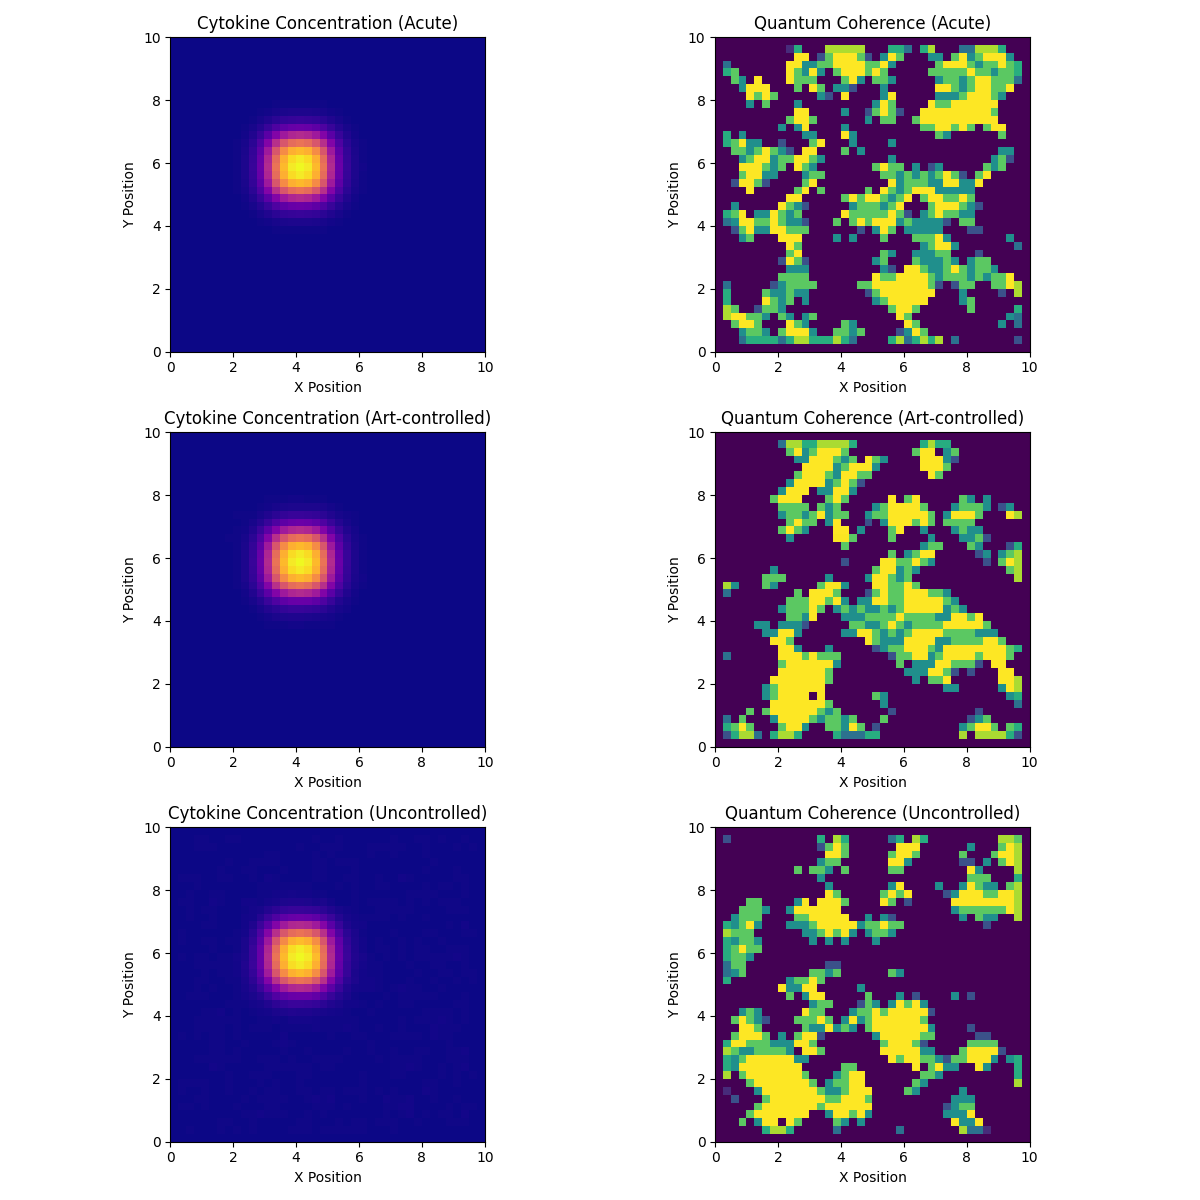
\includegraphics[width=0.8\textwidth]{Microtubule_Simulation/figures/HIV_stochastic_concentration_dependent.png}
\caption{Time evolution of cytokine diffusion and corresponding coherence collapse in HAND. Acute immune activation leads to localized coherence loss, while chronic low-level inflammation results in cumulative coherence degradation.}
\label{fig:HIV_coherence_collapse}
\end{figure}

\begin{figure}[H]
\centering
\includegraphics[width=0.8\textwidth]{Microtubule_Simulation/figures/HIV_cytokine_coherence_evolution.png}
\caption{Simulated quantum coherence loss in HAND. Progressive degradation of coherence over time corresponds to increasing TNF-α, IL-6, and IL-1β concentrations.}
\label{fig:HIV_wavefunction_evolution}
\end{figure}
\end{document}